\documentclass[../main.tex]{subfiles}
\begin{document}
\section{Appendix to Chapter 2}

\subsection{A review of complex analysis basics}
\begin{theorem}[Cauchy's integral formula]
  For an analytic function $f(z)=\sum_{n=0}^{\infty} a_n z^n$ on a disk $|z|<R$,
  \begin{equation}
    a_n = \frac{f^{(n)}(0)}{n!} = \frac{1}{2\pi i} \int_{|z|=r} \frac{f(z)}{z^{n+1}} \, dz
  \end{equation}
\end{theorem}

\begin{definition}[Complex logarithm]
  \begin{equation}
    \log z := \ln r + i\theta \quad (z=re^{i\theta}, \; r>0, \; \theta \in (-\pi, \pi])
  \end{equation}
  Remind that $\log z$ is not continuous on the negative real axis.
\end{definition}

\begin{proposition}
  Let $R$ be the ray $\{ xe^{i\theta} \mid x \in [0, \infty) \}$ for a fixed $\theta$.
  If $F$ is an analytic function such that $|F(z)| = \mathcal{O}(|z|^{-2})$ then
  $\int_{R} F(z) \, dz = \int_{0}^{\infty} F(x) \, dx$
\end{proposition}
\begin{proof}
  Let $C_r$ be the circular arc $\{ re^{i\varphi} \mid \varphi \in [0, \theta] \}$.
  By Cauchy's theorem, $\int_{0}^{r} F(x) \, dx + \int_{C_r} F(z) \, dz - \int_{R_r} F(z) \, dz = 0$ where $R_r = \{ xe^{i\theta} \mid x \in [0, r] \}$.
  As $r \to \infty$, $\int_{C_r} F(z) \, dz = \int_{0}^{2\pi} F(re^{i\varphi}) \, ird\varphi \ll \frac{2\pi M}{r} \to 0$.
  Therefore, $\int_{0}^{\infty} F(x) \, dx - \int_{R} F(z) \, dz = 0$.
\end{proof}
The function in interest in chapter 2 is $F(z) = \frac{1}{z}\left(\frac{1}{e^{z} - 1}-\frac{1}{z}+\frac{e^{-z}}{2}\right)$.
When $z\gg 0$, $\frac{1}{z}$ dominates the other two terms in the parenthesis, so $|F(z)| \ll \frac{1}{|z|^{2}}$.

\subsection{Riemann Sums}
\begin{theorem}
  Let $\phi$ be a continuous decreasing function on $(0, \infty)$ and $\int_0^{\infty} \phi(x) \, dx$ converges. Then,
  \begin{equation*}
    -\phi(0)h \le \sum_{k=0}^{\infty} \phi(kh)h - \int_0^{\infty} \phi(x) \, dx \le \phi(0)h
  \end{equation*}
\end{theorem}

\begin{figure}[ht]
  \centering

  \begin{minipage}{0.48\textwidth}
    \centering
    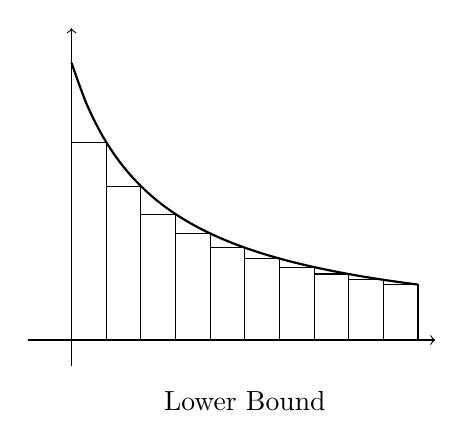
\begin{tikzpicture}[scale=1.1]
      \draw[->] (-0.5,0) -- (4.2,0);
      \draw[->] (0,-0.3) -- (0,3.6);

      \draw[domain=0:4,smooth,thick] plot (\x,{3.2/(1+\x)});

      \def\dx{0.4}
      \foreach \i in {0,...,9} {
          \pgfmathsetmacro\x{\i*\dx}
          \pgfmathsetmacro\h{3.2/(1+(\x+\dx))}
          \draw (\x,0) rectangle ++(\dx,\h);
        }
      \node at (2,-0.7) {Lower Bound};
    \end{tikzpicture}
  \end{minipage}
  \hfill
  \begin{minipage}{0.48\textwidth}
    \centering
    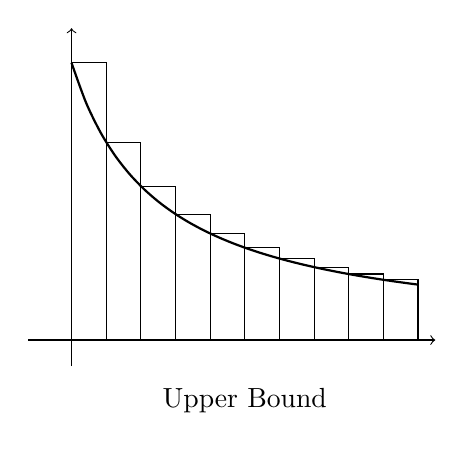
\begin{tikzpicture}[scale=1.1]
      \draw[->] (-0.5,0) -- (4.2,0);
      \draw[->] (0,-0.3) -- (0,3.6);

      \draw[domain=0:4,smooth,thick] plot (\x,{3.2/(1+\x)});

      \def\dx{0.4}
      \foreach \i in {0,...,9} {
          \pgfmathsetmacro\x{\i*\dx}
          \pgfmathsetmacro\h{3.2/(1+\x)}
          \draw (\x,0) rectangle ++(\dx,\h);
        }
      \node at (2,-0.7) {Upper Bound};
    \end{tikzpicture}
  \end{minipage}

\end{figure}

\begin{theorem}
  For a continuous real fuction $f$ on $(0, \infty)$, it can be written as a difference of two decreasing functions. Say $f= \phi - \psi$, Then
  \begin{equation*}
    -h(\phi(0) + \psi(0)) \le \sum_{k=0}^{\infty} f(kh)h - \int_0^{\infty} f(x) \, dx \le h(\phi(0) + \psi(0)) = hV(f)
  \end{equation*}
  Here $V(f)$ is the total variation of $f$ on $(0, \infty)$.
\end{theorem}

For a complex function $F=f+ig$, the theory continues as:
\begin{equation*}
  \begin{split}
    \left| \sum_{k=0}^{\infty} F(kh)h - \int_0^{\infty} F(x) \, dx \right| &\le \left| \sum_{k=0}^{\infty} f(kh)h - \int_0^{\infty} f(x) \, dx \right| \\
    &\quad + \left| \sum_{k=0}^{\infty} g(kh)h - \int_0^{\infty} g(x) \, dx \right| \\
    &\le h(V(f) + V(g)) = hV(F)
  \end{split}
\end{equation*}
Because it is tedious to write $||$ each time, we would invent a notation and rewrite the result as follows:
\begin{equation*}
  \sum_{k=0}^{\infty} F(kh)h - \int_0^{\infty} F(x) \, dx \ll hV(F)
\end{equation*}

\subsection{Dirty Calculations}
Let $F(z) = \frac{1}{z}\left(\frac{1}{e^{z} - 1}-\frac{1}{z}+\frac{e^{-z}}{2}\right)$. With some terrible calculations, 
\begin{equation*}
  \begin{split}
  F'(xe^{i\theta}) &= \frac{2}{x^3 e^{3i\theta}} - \frac{e^{-xe^{i\theta}}}{2x^2 e^{2i\theta}} - \frac{e^{-xe^{i\theta}}}{2xe^{i\theta}} \\
  &\quad - \frac{e^{xe^{i\theta}}}{x^2 e^{2i\theta}(e^{xe^{i\theta}} - 1)} - \frac{e^{xe^{i\theta}}}{xe^{i\theta}(e^{xe^{i\theta}} - 1)^2}
  \end{split}
\end{equation*}

Observe $(e^{xe^{i\theta}} - 1) \sim e^{xe^{i\theta}} \gg x^{m}$ if $\Re(xe^{i\theta}) > 0$ i.e. $\theta \in (-\frac{\pi}{2}, \frac{\pi}{2})$.
Now you should be able to briefly grasp that $|F'(xe^{i\theta})| \ll \frac{1}{x^2}$ in any wedge $|\theta| < c < \frac{\pi}{2}$ except some near $x=0$.

\begin{equation*}
  V_{\theta}(F) = \int_0^{\infty} |F'(xe^{i\theta})| \, dx = c_{1} + \int_{c_{2}}^{\infty} |F'(xe^{i\theta})| \, dx \ll c_{1} + \int_{c_{2}}^{\infty} \frac{1}{x^2} \, dx = c_{1} + \frac{1}{c_{2}}
\end{equation*}

So, $w\cdot V_{\theta}(F) \ll Mw$. Here $c, c_{1}, c_{2}, M$ are some appropriate constants.
\end{document}
